\textbf{Feedback linearization} is an appproach to nonlinear control whose \textbf{central idea} is to algebraically transform a nonlinear system dynamics into a linear one, so that the well-known strategies for linear controllers could be applied. This technique differs from \textit{Jacobian linearization}, in the sense that the \textbf{linearization} is achieved by \textbf{exact} state transformation and feedback, instead of \textit{linear approximation} of the dynamics.\\

This idea of simplifying the form of the system's dynamics by choosing a different \textbf{state representation} is not unfamiliar, it is well known that in mechanics the description could vary a lot according to the choice of the \textbf{reference frame} or \textbf{coordinate system}.  \\

In the introductory discussion of feedback linearization, commonly one give the example of designing a control law for controlling the \textbf{fluid entering into a tank}. Given the dynamics, it is  quite simple to show that can be chosen a particularly simple input to delete the non linearities of the plant in a way that the system resulting in a simple \textbf{integrator}.\\
In more complex situations, than the tank system, it is required to have some standard techniques to linearize the system. In this context we can mention:
\begin{enumerate}
    \item \textbf{input-state linearization} where linearization is performed via state feedback; 
    \item \textbf{input-output} linearization, here linearization is achieved by using the feedback of the output.
\end{enumerate}

To this aim it is useful to introduce the concept of \textbf{Lie derivatives} which is an elegant way to express the well-known \textbf{chain rule}. 
\section{Lie derivatives}
This definitions are given in order to use a more compact notation for the following paragraphs. \\

\hspace*{-5mm}
\begin{tikzpicture}
\node [mybox] (box){%
    \begin{minipage}{.96\textwidth}     %Larghezza del box
          \textbf{Definition} A function $f(x)$ is said to be \textbf{smooth} if it has continuous partial derivatives of any required order.
    \end{minipage}
};
\end{tikzpicture}% 

\vspace{0.5cm}
\hspace*{-5mm}
\begin{tikzpicture}
\node [mybox] (box){%
    \begin{minipage}{.96\textwidth}     %Larghezza del box
          \textbf{Definition} Let $h:\mathbb{R}^n\rightarrow \mathbb{R}$ a smooth function, and $f:\mathbb{R}^n\rightarrow\mathbb{R}^n$ a \textit{vector field} of $\mathbb{R}^n$. The \textbf{Lie Derivative of $h$ with respect to $f$} is a scalar function defined by $L_fh\doteq\nabla h f \in \mathbb{R}$
    \end{minipage}
};
\end{tikzpicture}%

\noindent
The meaning of \textbf{Lie derivative} is doing a derivative of $h$ in the direction provided by $f$. The computation of such derivatives can be done in a \textbf{recursive way}, as follows: 
\begin{align*}
    &L_f^0h=h\\
    &L_f^ih=L_f(L_f^{i-1}h)=\nabla(L_f^{i-1}h)f, \quad i=1, 2, ...
\end{align*}

\section{Input-Output linearization}
Now we consider the \textbf{SISO nonlinar system} of the form 
\begin{equation} \label{eq: system_affine}
    \begin{aligned}
        &\dot{x} = f(x)+g(x)u\\
        &y=h(x)
\end{aligned}
\end{equation}

where $x\in\mathbb{R}^{n_x}$ is the state, $u\in\mathbb{R}$ is the command input, $y\in\mathbb{R}$ is the output, and $f$, $g$, $h$ are smooth functions.\\
Such system is said to be \textit{affine in u}. We assume that the state is accessible and so measurable, otherwise an observer has to be employed. \\
\textbf{Input-output linearization} approach consists in differentiate repeatedly, until the input $u$ appears, then design the control law $u(t)$ to cancel the nonlinearity.\\
We can start by taking the output equation $y=h(x)$ and differentiate it: 
\begin{align}
    &\dot{y}=\frac{\partial h}{\partial x}\dot{x}=\nabla h(x)\dot{x}=
    \nabla h(x) (f(x)+g(x)u) = \\
    &\nabla h(x) f(x) + \nabla h(x) g(x) u=
    L_fh+L_gh(x)u
\end{align}
If $L_gh(x) \ne 0$ at some point $x=\bar{x}\in \Omega_x\subseteq\mathbb{R}^n$ then in $\Omega_x$ the control law is: 
\begin{equation}
    u=\frac{1}{L_gh(x)} (-L_fh(x)+v)
\end{equation}
This transforms the output equation in $\dot{y}=v$. Otherwise we differentiate again obtaining: 
\begin{align}
    \ddot{y}=L_f^2h(x)+L_gL_fh(x)u
\end{align}
Until the multiplicative term of $u$ is not null, you have to differentiate again and again obtaining:
\begin{equation}
    y^{(i)}=L_f^{(i)}h(x)+L_gL_f^{(i-1)}h(x)u
\end{equation}
Then, for some $\gamma$ the term $L_gL_f^{\gamma-1}h(x)u \ne 0$ the control law and the resulting system will be respectively\\


\hspace*{-5mm}
\begin{tikzpicture}
\node [mybox] (box){%
    \begin{minipage}{.96\textwidth}     %Larghezza del box
    {
        \large{
         \begin{align}
    &u=\frac{1}{L_gL_f^{\gamma}h(x)}(-L_f^{\gamma-1}+v)\\
    &y^{(\gamma)}=v \label{eq: final_system}
\end{align}}
}
    \end{minipage}
};
\end{tikzpicture}%


The equation (\ref{eq: final_system}) can be written in the state space form, definining the \textbf{state vector}
\begin{equation}
    \mu=(\mu_1,...,\mu_\gamma)\doteq(y, \dot{y},...,y^{(\gamma-1)})
\end{equation}
The resulting state equations are in the so-called \textit{companion form}: \\

\hspace*{-5mm}
\begin{tikzpicture}
\node [mybox] (box){%
    \begin{minipage}{.96\textwidth}     %Larghezza del box
    {
        \large{
         \begin{align*}
    &\dot{\mu}=A\mu+Bv\\
    &y=\mu_1\\
    &A=\begin{bmatrix}
    0&1&0&\dots&0\\
    0&0&1&\ddots&0\\
    \vdots&\vdots&\ddots&\ddots&\vdots\\
    0&0&\dots&0&1\\
    0&0&\dots&0&0
    \end{bmatrix} \quad 
    B=\begin{bmatrix}
        0\\0\\\vdots\\0\\1
    \end{bmatrix}
\end{align*}}
}
    \end{minipage}
};
\end{tikzpicture}%


These equations describe only a part of the system dynamics, called the {\textbf{external dynamics}}, which is the part that one can control. This is linked with another important information of the non linear system that is the \textbf{relative degree}.

\subsection{Relative degree}
Now we give the definition of \textbf{relative degree}:\\

\hspace*{-5mm}
\begin{tikzpicture}
\node [mybox] (box){%
    \begin{minipage}{.96\textwidth}     %Larghezza del box
    \textbf{Definition } The integer $\gamma\le n$ is the \textbf{relative degree} of the system (\ref{eq: system_affine}) in $\Omega$.
    \end{minipage}
};
\end{tikzpicture}% 
\\

 This is a generalization of the concept of relative degree for LTI systems (the difference between the denominator degree and numerator degree of the transfer function $H(s).$
 In the case that $\gamma=n$, input-output linearization corresponds to input-state linearization.\\
 It could happen that the term $L_gL_f^{\gamma-1}h(x)$ is zero at $\bar{x}$ but non zero in the neighbourhood of $\bar{x}$.
 In this case the relative degree is \textit{undefined} in $\bar{x}$.
 
 \subsection{Normal form}
Once we have applied the control law, we can define the \textbf{normal state} $(\mu,\psi)$ in the following way:
\begin{align}
    &\mu=(\mu_1, ..., \mu_\gamma)\doteq (y, \dot{y},..., y^{\gamma-1})\in\mathbb{R}^{\gamma} \quad & \text{external dynamics}\\
    &\psi\in\mathbb{R}^{n-\gamma} & \text{internal dynamics}
\end{align}
The nonlinear system (\ref{eq: system_affine}) can be written in the so called \textit{normal form}:
\begin{equation}
    \begin{aligned}
        &\dot{\mu}=\begin{bmatrix}
            \mu_2\\
            \vdots\\
            \mu_\gamma\\
            a(\mu, \psi)+b(\mu,\psi)u
        \end{bmatrix} \quad \begin{matrix}
            &a(\mu, \psi)\doteq L_f^{\gamma}h(x)\\
            &b(\mu, \psi)\doteq L_gL_f^{\gamma-1}h(x)u
        \end{matrix}\\
        &\dot{\psi}=w(\mu,\psi)\\
        &y=\mu_1
    \end{aligned}
\end{equation}
While the \textbf{external dynamics} is well defined and one can control it, find explicitly the \textbf{internal dynamics} could require to solve Partial Differential Equations (PDE), however in some cases it is possible to study the \textbf{stability of the internal dynamics} theoretically by using the \textit{zero dynamics} otherwise simulations have to be used.
 
\subsection{Zero dynamics}
The internal dynamics of the system (\ref{eq: system_affine}) is not controlled, it can be therefore either bounded or unbounded. We introduce the concept of \textbf{zero dynamics} which represents a simplification of the internal dynamics.\\

\hspace*{-5mm}
\begin{tikzpicture}
\node [mybox] (box){%
    \begin{minipage}{.96\textwidth}     %Larghezza del box
    \textbf{Definition (Zero dynamics)} The zero-dynamics of the system \ref{eq: system_affine} in $\Omega$ is defined by 
    \begin{equation} \label{eq: zero_dyn}
        \begin{aligned}
            &\dot{\mu}=0\\
            &\psi=w(0,\psi)
        \end{aligned}
    \end{equation}
    with initial conditions $\mu(0)=0$ and $\psi(0)=\psi_0$
    \end{minipage}
};
\end{tikzpicture}%

\vspace{0.2cm}
\hspace*{-5mm}
\begin{tikzpicture}
\node [mybox] (box){%
    \begin{minipage}{.96\textwidth}     %Larghezza del box
    \textbf{Definition} The system \ref{eq: system_affine} is \textit{locally asymptotically minimum phase at $\bar{x}$} if $\psi=0$ is a locally asymptotically stable equilibrium point of the system (\ref{eq: zero_dyn})
     \end{minipage}
};
\end{tikzpicture}%

\subsection{First control problem: Regulation}
In the introduction, we have seen that the most common problem in the field of automatic control are: regulation and tracking.\\
In order to obtain a \textbf{regulation} of the system (\ref{eq: system_affine}) is sufficient to define the control law:
\begin{equation}\label{eq:regulation}
    \begin{aligned}
        &u=\frac{1}{L_gL_f^{\gamma-1}h(x)u}(-L_gh(x)+v) &\text{feedback linearization}\\
        &v=-K\mu &{\color{red}{\text{linear control}}}
    \end{aligned}
\end{equation}
where $K=[k_1,..., k_\gamma]\in\mathbb{R}^\gamma$ is such that $A-BK$ is asymptotically stable. \\

\hspace*{-5mm}
\begin{tikzpicture}
\node [mybox] (box){%
    \begin{minipage}{.96\textwidth}     %Larghezza del box
    \textbf{Theorem} Assume that the system (\ref{eq: system_affine}) has a locally asymptotically stable zero dynamics. Then, the \textit{closed loop} defined by (\ref{eq: system_affine}) and (\ref{eq:regulation}) is \textit{locally asymptotically stable}.
    \end{minipage}
};
\end{tikzpicture}%
\subsection{Second control problem: Tracking}
Now let consider the problem that the system output is required to track a desired signal $r(t)$, this signal has to be \textbf{smooth} and \textbf{bounded}. Let $\mu_r\doteq(r,\dot{r},..., r^{\gamma-1})$, we define the \textbf{tracking error} as
$$\Tilde{\mu}\doteq\mu_r-\mu$$
We would like to make this error small and possibly to force it to converge to zero. Even in this case we define: 
\begin{equation}\label{eq:tracking}
    \begin{aligned}
        &u=\frac{1}{L_gL_f^{\gamma-1}h(x)u}(-L_gh(x)+v) &\text{feedback linearization}\\
        &v=-K\Tilde{\mu}+r^{(\gamma)} &\text{linear control}
    \end{aligned}
\end{equation}
where $K=[k_1,..., k_\gamma]\in\mathbb{R}^\gamma$ is such that $A-BK$ is asymptotically stable. \\

\hspace*{-5mm}
\begin{tikzpicture}
\node [mybox] (box){%
    \begin{minipage}{.96\textwidth}     %Larghezza del box
    \textbf{Theorem} Assume that the solution of the equation 
    $$\dot{\psi_r}=w(\mu_r, \psi_r), \quad \psi_r(0)=0$$
    exists, and is bounded and asymptotically stable. The, $\Tilde{\mu}(t)$ converges exponentially  to 0, as $t \rightarrow \infty$
    \end{minipage}
};
\end{tikzpicture}%

\subsection{Control scheme}
The aim of this section is to give a general control scheme for physical systems/plants controlled by using the \textit{feedback linearization}.  

\begin{figure}[h]
    \centering
    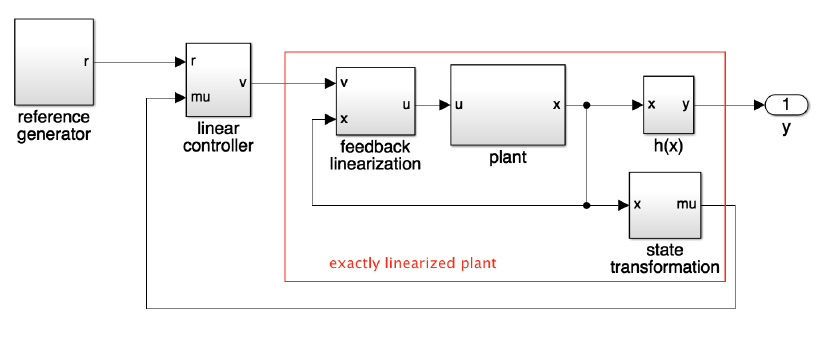
\includegraphics[scale=0.7]{NonLinearControl/images/FL_ControlScheme .png}
    \caption{Feedback linearization control scheme}
    \label{fig:FL_controlscheme}
\end{figure}

Now we are going to describe the blocks of the figure (\ref{fig:FL_controlscheme}):
\begin{itemize}
    \item \textbf{Plant}: is a nonlinear system affine in the input u of the form $\dot{x}=f(x)+g(x)u$;
    \item \textbf{State transformation}: is obtained by applying $\mu=(y, \dot{y}, ..., y^{(\gamma-1)})=(h(x), L_fh(x), ..., L_f^{\gamma-1}h(x))$
    \item \textbf{Feedback linearization}: is obtained implementing the equation \ref{eq:tracking}; 
    \item The \textbf{linear controller} can be implemented by using any technique (eg. pole placement)
\end{itemize}

\section{Discussion}
It is useful pay attention that:
\begin{enumerate}
    \item The results which has been found for Feedback linearization hold in \textit{some region} of the state space $\Omega\subseteq\mathbb{R}^n$, in particular where the multiplicative term $L_gL_f^{\gamma-1}h(x)$ is non-zero. Global results are available but we have to do stronger assumptions.
    \item We have seen that there are relevant differences with respect to \textbf{Conventional linearization}: in FL the linearization is exact on the whole region $\Omega$. Even in the case the CL worked, the Feedback linearization gives better results; 
    \item The Feedback linearization technique does not take into account problems related to the uncertainty of the nominal plant and parameters: issue linked to the robustness are provided instead by other techniques like \textit{sliding mode control}.
\end{enumerate}